%% (Master) Thesis template
% Template version used: v1.4
%
% Largely adapted from Adrian Nievergelt's template for the ADPS
% (lecture notes) project.


%% We use the memoir class because it offers a many easy to use features.
\documentclass[11pt,a4paper,titlepage,dvipsnames]{memoir}

%% Packages
%% ========

%% LaTeX Font encoding -- DO NOT CHANGE
\usepackage[OT1]{fontenc}

%% Babel provides support for languages.  'english' uses British
%% English hyphenation and text snippets like "Figure" and
%% "Theorem". Use the option 'ngerman' if your document is in German.
%% Use 'american' for American English.  Note that if you change this,
%% the next LaTeX run may show spurious errors.  Simply run it again.
%% If they persist, remove the .aux file and try again.
\usepackage[english]{babel}

%% Input encoding 'utf8'. In some cases you might need 'utf8x' for
%% extra symbols. Not all editors, especially on Windows, are UTF-8
%% capable, so you may want to use 'latin1' instead.
\usepackage[utf8]{inputenc}

%% This changes default fonts for both text and math mode to use Herman Zapfs
%% excellent Palatino font.  Do not change this.
\usepackage[sc]{mathpazo}

%% The AMS-LaTeX extensions for mathematical typesetting.  Do not
%% remove.
\usepackage{amsmath,amssymb,amsfonts,mathrsfs}

%% NTheorem is a reimplementation of the AMS Theorem package. This
%% will allow us to typeset theorems like examples, proofs and
%% similar.  Do not remove.
%% NOTE: Must be loaded AFTER amsmath, or the \qed placement will
%% break
\usepackage[amsmath,thmmarks]{ntheorem}

%% LaTeX' own graphics handling
\usepackage{graphicx}

%% We unfortunately need this for the Rules chapter.  Remove it
%% afterwards; or at least NEVER use its underlining features.
\usepackage{soul}

%% This allows you to add .pdf files. It is used to add the
%% declaration of originality.
\usepackage{pdfpages}

%% For the epigraph of chapters.
\usepackage{epigraph}

%% Subfigures
\usepackage{caption,subcaption}

%% Some more packages that you may want to use.  Have a look at the
%% file, and consult the package docs for each.
%% See the TeXed file for more explanations

%% [OPT] Multi-rowed cells in tabulars
%\usepackage{multirow}

%% [REC] Intelligent cross reference package. This allows for nice
%% combined references that include the reference and a hint to where
%% to look for it.
\usepackage{varioref}

%% [OPT] Easily changeable quotes with \enquote{Text}
%\usepackage[german=swiss]{csquotes}

%% [REC] Format dates and time depending on locale
\usepackage{datetime}

%% [OPT] Provides a \cancel{} command to stroke through mathematics.
%\usepackage{cancel}

%% [NEED] This allows for additional typesetting tools in mathmode.
%% See its excellent documentation.
\usepackage{mathtools}

%% [ADV] Conditional commands
%\usepackage{ifthen}

%% [OPT] Manual large braces or other delimiters.
%\usepackage{bigdelim, bigstrut}

%% [REC] Alternate vector arrows. Use the command \vv{} to get scaled
%% vector arrows.
\usepackage[h]{esvect}

%% [NEED] Some extensions to tabulars and array environments.
\usepackage{array}

%% [OPT] Postscript support via pstricks graphics package. Very
%% diverse applications.
%\usepackage{pstricks,pst-all}

%% [?] This seems to allow us to define some additional counters.
%\usepackage{etex}

%% [ADV] XY-Pic to typeset some matrix-style graphics
%\usepackage[all]{xy}

%% [OPT] This is needed to generate an index at the end of the
%% document.
%\usepackage{makeidx}

%% [OPT] Fancy package for source code listings.  The template text
%% needs it for some LaTeX snippets; remove/adapt the \lstset when you
%% remove the template content.
\usepackage{listings}
\lstset{language=TeX,basicstyle={\normalfont\ttfamily}}

%% [REC] Fancy character protrusion.  Must be loaded after all fonts.
\usepackage{microtype}

%% [REC] Nicer tables.  Read the excellent documentation.
\usepackage{booktabs}

\usepackage{todonotes}
\newcommand{\pengcheng}[1]{\todo[color=LimeGreen, inline]{\textbf{pengcheng: }#1}}
\newcommand{\pengxu}[1]{\pengcheng{1}}

% https://tex.stackexchange.com/a/9372
\newcommand{\mytilde}{\raise.17ex\hbox{$\scriptstyle\mathtt{\sim}$}}

% https://tex.stackexchange.com/questions/42619/xmark-that-complements-the-ams-checkmark
\newcommand{\yes}{{\bf\ding{51}}}
\newcommand{\partially}{{\bf\ding{108}}}
\newcommand{\no}{{\bf\ding{55}}}

% http://identitystandards.acm.org/identitystandards.pdf
\definecolor{acmred}{RGB}{253,27,20}
\definecolor{acmgreen}{RGB}{166,188,9}
\definecolor{acmyellow}{RGB}{255,214,0}


%% Our layout configuration.  DO NOT CHANGE.
%% Memoir layout setup

%% NOTE: You are strongly advised not to change any of them unless you
%% know what you are doing.  These settings strongly interact in the
%% final look of the document.

% Dependencies
\usepackage{ETHlogo}

% Turn extra space before chapter headings off.
\setlength{\beforechapskip}{0pt}

\nonzeroparskip
\parindent=0pt
\defaultlists

% Chapter style redefinition
\makeatletter

\if@twoside
  \pagestyle{Ruled}
  \copypagestyle{chapter}{Ruled}
\else
  \pagestyle{ruled}
  \copypagestyle{chapter}{ruled}
\fi
\makeoddhead{chapter}{}{}{}
\makeevenhead{chapter}{}{}{}
\makeheadrule{chapter}{\textwidth}{0pt}
\copypagestyle{abstract}{empty}

\makechapterstyle{bianchimod}{%
  \chapterstyle{default}
  \renewcommand*{\chapnamefont}{\normalfont\Large\sffamily}
  \renewcommand*{\chapnumfont}{\normalfont\Large\sffamily}
  \renewcommand*{\printchaptername}{%
    \chapnamefont\centering\@chapapp}
  \renewcommand*{\printchapternum}{\chapnumfont {\thechapter}}
  \renewcommand*{\chaptitlefont}{\normalfont\huge\sffamily}
  \renewcommand*{\printchaptertitle}[1]{%
    \hrule\vskip\onelineskip \centering \chaptitlefont\textbf{\vphantom{gyM}##1}\par}
  \renewcommand*{\afterchaptertitle}{\vskip\onelineskip \hrule\vskip
    \afterchapskip}
  \renewcommand*{\printchapternonum}{%
    \vphantom{\chapnumfont {9}}\afterchapternum}}

% Use the newly defined style
\chapterstyle{bianchimod}

\setsecheadstyle{\Large\bfseries\sffamily}
\setsubsecheadstyle{\large\bfseries\sffamily}
\setsubsubsecheadstyle{\bfseries\sffamily}
\setparaheadstyle{\normalsize\bfseries\sffamily}
\setsubparaheadstyle{\normalsize\itshape\sffamily}
\setsubparaindent{0pt}

% Set captions to a more separated style for clearness
\captionnamefont{\sffamily\bfseries\footnotesize}
\captiontitlefont{\sffamily\footnotesize}
\setlength{\intextsep}{16pt}
\setlength{\belowcaptionskip}{1pt}

% Set section and TOC numbering depth to subsection
\setsecnumdepth{subsection}
\settocdepth{subsection}

%% Titlepage adjustments
\pretitle{\vspace{0pt plus 0.7fill}\begin{center}\HUGE\sffamily\bfseries}
\posttitle{\end{center}\par}
\preauthor{\par\begin{center}\let\and\\\Large\sffamily}
\postauthor{\end{center}}
\predate{\par\begin{center}\Large\sffamily}
\postdate{\end{center}}

\def\@advisors{}
\newcommand{\advisors}[1]{\def\@advisors{#1}}
\def\@department{}
\newcommand{\department}[1]{\def\@department{#1}}
\def\@thesistype{}
\newcommand{\thesistype}[1]{\def\@thesistype{#1}}

\renewcommand{\maketitlehooka}{\noindent\ETHlogo[2in]}

\renewcommand{\maketitlehookb}{\vspace{1in}%
  \par\begin{center}\Large\sffamily\@thesistype\end{center}}

\renewcommand{\maketitlehookd}{%
  \vfill\par
  \begin{flushright}
    \sffamily
    \@advisors\par
    \@department, ETH Z\"urich
  \end{flushright}
}

\checkandfixthelayout

\setlength{\droptitle}{-48pt}

\makeatother

% This defines how theorems should look. Best leave as is.
\theoremstyle{plain}
\setlength\theorempostskipamount{0pt}

%%% Local Variables:
%%% mode: latex
%%% TeX-master: "thesis"
%%% End:


%% Theorem environments.  You will have to adapt this for a German
%% thesis.
%% Theorem-like environments

%% This can be changed according to language. You can comment out the ones you
%% don't need.

\numberwithin{equation}{chapter}

%% German theorems
%\newtheorem{satz}{Satz}[chapter]
%\newtheorem{beispiel}[satz]{Beispiel}
%\newtheorem{bemerkung}[satz]{Bemerkung}
%\newtheorem{korrolar}[satz]{Korrolar}
%\newtheorem{definition}[satz]{Definition}
%\newtheorem{lemma}[satz]{Lemma}
%\newtheorem{proposition}[satz]{Proposition}

%% English variants
\newtheorem{theorem}{Theorem}[chapter]
\newtheorem{example}[theorem]{Example}
\newtheorem{remark}[theorem]{Remark}
\newtheorem{corollary}[theorem]{Corollary}
\newtheorem{definition}[theorem]{Definition}
\newtheorem{lemma}[theorem]{Lemma}
\newtheorem{proposition}[theorem]{Proposition}

%% Proof environment with a small square as a "qed" symbol
\theoremstyle{nonumberplain}
\theorembodyfont{\normalfont}
\theoremsymbol{\ensuremath{\square}}
\newtheorem{proof}{Proof}
%\newtheorem{beweis}{Beweis}


%% Helpful macros.
%% Custom commands
%% ===============

%% Special characters for number sets, e.g. real or complex numbers.
\newcommand{\C}{\mathbb{C}}
\newcommand{\K}{\mathbb{K}}
\newcommand{\N}{\mathbb{N}}
\newcommand{\Q}{\mathbb{Q}}
\newcommand{\R}{\mathbb{R}}
\newcommand{\Z}{\mathbb{Z}}
\newcommand{\X}{\mathbb{X}}

%% Fixed/scaling delimiter examples (see mathtools documentation)
\DeclarePairedDelimiter\abs{\lvert}{\rvert}
\DeclarePairedDelimiter\norm{\lVert}{\rVert}

%% Use the alternative epsilon per default and define the old one as \oldepsilon
\let\oldepsilon\epsilon
\renewcommand{\epsilon}{\ensuremath\varepsilon}

%% Also set the alternate phi as default.
\let\oldphi\phi
\renewcommand{\phi}{\ensuremath{\varphi}}

% comments
\newcommand{\pengcheng}[1]{\todo[color=LimeGreen, inline]{\textbf{pengcheng: }#1}}
\newcommand{\pengxu}[1]{\pengcheng{#1}}

% https://tex.stackexchange.com/a/9372
\newcommand{\mytilde}{\raise.17ex\hbox{$\scriptstyle\mathtt{\sim}$}}

% https://tex.stackexchange.com/questions/42619/xmark-that-complements-the-ams-checkmark
\newcommand{\yes}{{\bf\ding{51}}}
\newcommand{\partially}{{\bf\ding{108}}}
\newcommand{\no}{{\bf\ding{55}}}


%% Acronyms.
\usepackage{acro}
\usepackage{multicol}

%\acsetup{make-links}
\acsetup{format/first-long=\itshape}
\DeclareAcronym{pe}{
  short=PE,
  long=processing element,
}
\DeclareAcronym{soc}{
  short=SoC,
  long=system-on-chip,
}
\DeclareAcronym{fpga}{
  short=FPGA,
  long=field-programmable gate array,
}
\DeclareAcronym{asic}{
  short=ASIC,
  long=application-specific integrated circuit,
}
\DeclareAcronym{spin}{
  short=sPIN,
  long=streaming Processing in the Network,
}
\DeclareAcronym{nisa}{
  short=NISA,
  long=network instruction set architecture,
}
\DeclareAcronym{isa}{
  short=ISA,
  long=instruction set architecture,
}
\DeclareAcronym{hpu}{
  short=HPU,
  long=handler processing unit,
}
\DeclareAcronym{dma}{
  short=DMA,
  long=direct memory access,
}
\DeclareAcronym{clb}{
  short=CLB,
  long=configurable logic block,
}
\DeclareAcronym{lut}{
  short=LUT,
  long=look-up table,
}
\DeclareAcronym{ff}{
  short=FF,
  long=flip-flop,
}
\DeclareAcronym{bram}{
  short=BRAM,
  long=block RAM,
}
\DeclareAcronym{uram}{
  short=URAM,
  long=Ultra RAM,
}
\DeclareAcronym{sta}{
  short=STA,
  long=static timing analysis,
}
\DeclareAcronym{eda}{
  short=EDA,
  long=electronic design automation,
}
\DeclareAcronym{wns}{
  short=WNS,
  long=worst negative slack,
}
\DeclareAcronym{whs}{
  short=WHS,
  long=worst hold slack,
}
\DeclareAcronym{tns}{
  short=TNS,
  long=total negative slack,
}
\DeclareAcronym{ths}{
  short=THS,
  long=total hold slack,
}
\DeclareAcronym{ip}{
  short=IP,
  long=intellectual property,
}
\DeclareAcronym{axi}{
  short=AXI,
  long=Advanced eXtensible Interface,
}
\DeclareAcronym{cma}{
  short=CMA,
  long=Contiguous Memory Allocator,
}
\DeclareAcronym{mpq}{
  short=MPQ,
  long=message processing queue,
}
\DeclareAcronym{qor}{
  short=QoR,
  long=quality of results,
}
\DeclareAcronym{her}{
  short=HER,
  long=handler execution request,
}
\DeclareAcronym{pblock}{
  short=PBlock,
  long=placement block,
}
\DeclareAcronym{dac}{
  short=DAC,
  long=direct-attached copper,
}
\DeclareAcronym{pulp}{
  short=PULP,
  long=PULP Ultra Low Power,
}
\DeclareAcronym{udp}{
  short=UDP,
  long=User Diagram Protocol,
}
\DeclareAcronym{arp}{
  short=ARP,
  long=Address Resolution Protocol,
}
\DeclareAcronym{mtu}{
  short=MTU,
  long=maximum transmission unit,
}
\DeclareAcronym{tcp}{
  short=TCP,
  long=Transmission Control Protocol,
}
\DeclareAcronym{sctp}{
  short=SCTP,
  long=Stream Control Transmission Protocol,
}
\DeclareAcronym{dccp}{
  short=DCCP,
  long=Datagram Congestion Control Protocol,
}
\DeclareAcronym{ipg}{
  short=IPG,
  long=inter-packet gap,
}
\DeclareAcronym{qos}{
  short=QoS,
  long=quality of service,
}
\DeclareAcronym{icmp}{
  short=ICMP,
  long=Internet Control Message Protocol,
}
\DeclareAcronym{ack}{
  short=ACK,
  long=acknowledgement,
}
\DeclareAcronym{syn}{
  short=SYN,
  long=synchronisation,
}
\DeclareAcronym{slmp}{
  short=SLMP,
  long=sPIN Lightweight Messaging Protocol,
}
\DeclareAcronym{cdc}{
  short=CDC,
  long=clock domain crossing,
}
\DeclareAcronym{rdma}{
  short=RDMA,
  long=remote direct memory access,
}
\DeclareAcronym{bar}{
  short=BAR,
  long=base address register,
}
\DeclareAcronym{mac}{
  short=MAC,
  long=media access control,
}
\DeclareAcronym{fifo}{
  short=FIFO,
  long=first-in first-out,
}
\DeclareAcronym{rtl}{
  short=RTL,
  long=register transfer level,
}
\DeclareAcronym{ila}{
  short=ILA,
  long=Integrated Logic Analyzer,
}
\DeclareAcronym{mpi}{
  short=MPI,
  long=Message Passing Interface,
}
\DeclareAcronym{poc}{
  short=PoC,
  long=proof of concept,
}
\DeclareAcronym{rq}{
  short=RQ,
  long=request queue,
}
\DeclareAcronym{cq}{
  short=CQ,
  long=completion queue,
}
\DeclareAcronym{nic}{
  short=NIC,
  long=network interface card,
}
\DeclareAcronym{pcie}{
  short=PCIe,
  long=Peripheral Component Interconnnect express,
}
\DeclareAcronym{eom}{
  short=EOM,
  long=end-of-message,
}
\DeclareAcronym{api}{
  short=API,
  long=application programming interface,
}
\DeclareAcronym{sdk}{
  short=SDK,
  long=software development kit,
}
\DeclareAcronym{img}{
  short=IMG,
  long=inter-message gap,
}
\DeclareAcronym{ipoib}{
  short=IPoIB,
  long=IP over InfiniBand,
}
\DeclareAcronym{e2e}{
  short=E2E,
  long=end-to-end,
}
\DeclareAcronym{rtt}{
  short=RTT,
  long=round-trip time,
}
\DeclareAcronym{gemm}{
  short=GEMM,
  long=general matrix multiply,
}
\DeclareAcronym{hpc}{
  short=HPC,
  long=high-performance computing,
}
\DeclareAcronym{rts}{
  short=RTS,
  long=request to send,
}
\DeclareAcronym{roce}{
  short=RoCE,
  long=RDMA over Converged Ethernet,
}

%% Make document internal hyperlinks wherever possible. (TOC, references)
%% This MUST be loaded after varioref, which is loaded in 'extrapackages'
%% above.  We just load it last to be safe.
\usepackage[linkcolor=black,colorlinks=true,citecolor=black,filecolor=black]{hyperref}

\usepackage{cleveref}

%\usepackage[outputdir=../]{minted}
\usepackage{minted}
\setminted{frame=lines, fontsize=\footnotesize, linenos, framesep=2mm}

%% Document information
%% ====================

\title{Full-System Evaluation of the sPIN In-Network-Compute Architecture}
\author{Pengcheng Xu}
\thesistype{Master Thesis}
\advisors{Advisors: Prof.\ Dr.\ Torsten Hoefler, Mikhail Khalilov, Timo Schneider}
\department{Department of Computer Science}
\date{September, 2023}

% for figures in background
\newlength{\twosubht}
\newsavebox{\twosubbox}

\begin{document}

\frontmatter

%% Title page is autogenerated from document information above.  DO
%% NOT CHANGE.
\begin{titlingpage}
  \calccentering{\unitlength}
  \begin{adjustwidth*}{\unitlength-24pt}{-\unitlength-24pt}
    \maketitle
  \end{adjustwidth*}
\end{titlingpage}

%% The abstract of your thesis.  Edit the file as needed.
\begin{abstract}
\pengcheng{What is in-network-computing, introduce sPIN and PsPIN}
PsPIN is the RISC-V-based packet processing cluster that implements the \acs{spin} in-network compute model proposed and developed at ETH Z{\"u}rich. 

\pengcheng{What composes a full SmartNIC}
While the design is fully synthesizable and comes with a cycle-accurate simulation model, it requires various other hardware and software components to function as a full system at realistic speeds. 

\pengcheng{FPsPIN; hardware and software system}
This project, FPsPIN, bridges the gap by developing a fully-functional demo FPGA SmartNIC based on PsPIN.  The demo system serves as a \acs{poc} for PsPIN in \acs{asic} and facilitates future software and hardware development of the \acs{spin} ecosystem.
\end{abstract}

\clearpage

\section*{Acknowledgements}

The author would like to thank...

%% TOC with the proper setup, do not change.
\cleartorecto
\tableofcontents
\mainmatter

%% Your real content!
% Some commands used in this file
\newcommand{\package}{\emph}

\chapter{Introduction}

\pengcheng{Concept of smartnic}
In recent years, the scaling potential of CPU-based networking stacks capacity gradually slowdowns compared to the NIC links due to hurdles of Moore's law scaling. SmartNIC is an emerging approach to increase networking throughput and reduce packet processing latency by combining compute cores with traditional NIC functionality. Existing SmartNIC architectures could be generally classified into two categories. The \textit{bump-in-the-wire} architecture comprises wimpy energy-efficient programmable cores placed within the NIC packet datapath. The \textit{side-band} architectures feature the SoC running a fully-fledged OS (e.g., Linux) that sees the NIC interface as a PCIe device.

A typical use-case of a SmartNIC is offloading the parts of user application that could be entirely done \textit{in the network}, e.g., gradient averaging in distributed deep learning. Thus, similarly to GPUs, SmartNICs need a hardware/software stack that could linearly scale with the data-arrival rates, a convenient API, and a management infrastructure that allows the users to benefit from in-network computing at the cost of \textit{minimal} changes to the application.

This project is a full end-to-end system demo of \underline{F}PGA-based \underline{PsPIN} SmartNIC~\cite{di2021risc} designed with a bump-in-the-wire architecture. We present the open-source hardware-software SmartNIC stack prototype capable of offloading various I/O and compute parts of the user applications using the sPIN programming model. We explain the hardware and software design of the FPsPIN system and showcase preliminary performance results in two real-world demo applications. While still a work in progress, the project already demonstrates the promising capabilities of sPIN-based SmartNIC in real life.

\begin{figure}
    \centering
    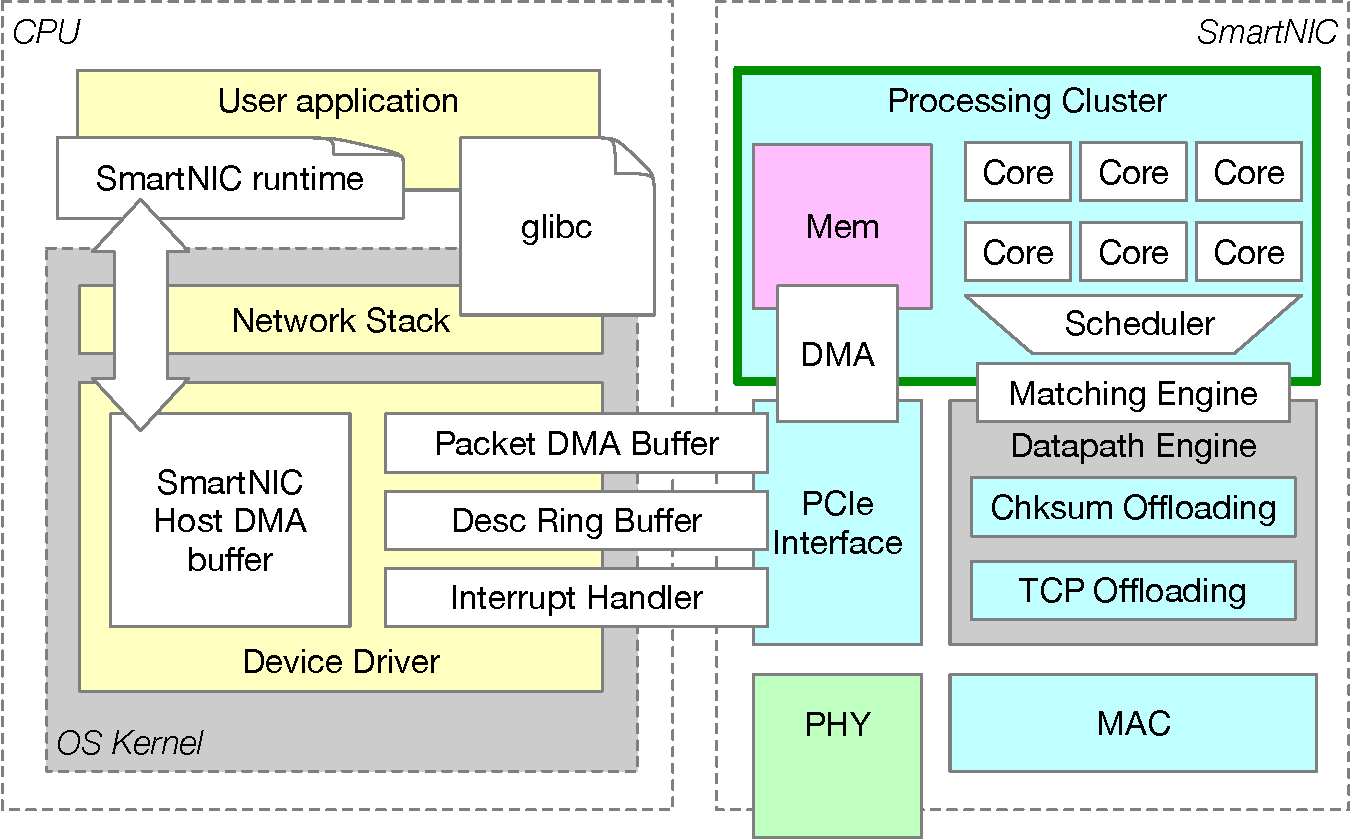
\includegraphics[width=.9\linewidth]{figures/system-overview.pdf}
    \caption{Overview of the complete server system, showing the software stack on the CPU and hardware components on the SmartNIC.  The green box marks the existing PsPIN processing cluster available from previous work.  Everything else needs to be developed, integrated and tested.}
    \label{fig:full-system}
\end{figure}
\chapter{Background}

\section{sPIN}
\pengcheng{sPIN in-network computing}
FPsPIN conforms to \underline{S}treaming \underline{P}rocessing \underline{i}n the \underline{N}etwork (sPIN). sPIN is a programming model that allows a programmer to offload lightweight data path and compute parts of the application code the NIC~\cite{hoefler2017spin}. sPIN is designed to expose packet level parallelism through execution of \textit{packet handlers}. Packet handlers are executed concurrently on the SmartNIC compute cores. sPIN defines three types of handlers that could be executed within the stateful context of a packet flow: 1) a header handler to be executed on the first packet of a flow, 2) a payload handler that is executed on every packet, and 3) a completion handler executed upon reception of the last packet.

\section{PsPIN} \label{sec:background-pspin}
\pengcheng{PsPIN}

\begin{table}[ht!]
\resizebox{\columnwidth}{!}{%
\begin{tabular}{@{}ccccc@{}}
\toprule
\textbf{Clusters, N}                                                                   & \textbf{2} & \textbf{4}    & \textbf{8} & \textbf{16} \\ \cmidrule(r){1-5}
Total Area, MGE                                                    & 45.25    & 90.50    & 181.00 & 362.01     \\ \addlinespace[0.5em]
Avg. Per-Packet Budget, Cycles                                                         & 346.05    & 692.10  & 1384.20 & 2768.38     \\\bottomrule
\end{tabular}%
}
\caption{Near linear scaling of the total cluster area ($8\times$ cores per cluster) compared to the per-packet time budget at $400$Gbit/s. The total area is estimated using synthesis of PsPIN in $22$nm@$1$GHz.}
\label{tab:cost_model}
\vspace{-0.9em}
\end{table}

FPsPIN is based on the PsPIN SmartNIC~\cite{di2021risc}, an open-source implementation of the sPIN API. PsPIN is a bump-in-the-wire SmartNIC architecture based on PULP, the silicon-proven energy-efficient 32-bit RISC-V SoC~\cite{rossi2015pulp}. Its memory hierarchy comprises shared per-cluster scratchpad memories that could be accessed in 1-cycle and slower L2 memory shared among core clusters.

\paragraph{PsPIN scalability} The key feature of PULP is its scalability, thanks to the hierarchical SoC interconnect based on the AXI protocol. As we report in \Cref{tab:cost_model}, the clustered architecture of PsPIN allows for a linear scaling of the SoC compute capacity compared to the total area needed for cores, memory, and SoC interconnect~\cite{di2021risc}. Thus, to fit a tighter per-packet processing budget with a higher link speed, one just needs to scale the number of PULP compute clusters proportionally. Estimation of a simulated per-packet time needed for offloading of the Reduce operation, a networking primitive that is used in distributed deep learning, shows that the optimal configuration at the 400 Gbit/s link bandwidth could be achieved at the 4 clusters, eight cores each.

\section{Corundum} \label{sec:background-corundum}
\pengcheng{Corundum: FPGA-based customizable 100G Ethernet NIC}

Corundum~\cite{forencich2020fccm} is an open-source, FPGA-based NIC and a platform for in-network computing.  The project supports 10/25/100 Gbps Ethernet on Xilinx and Intel platforms.  Among the many features it supports, the most important for FPsPIN is custom logic to extend the functionality of the NIC together with interfaces to the control path, data path, and DMA subsystems.  They also provide kernel drivers and user space utilities for Linux.  This makes it a perfect candidate platform for integrating a packet processing cluster to build a full SmartNIC.

\pengcheng{FPsPIN: bridge gaps between PsPIN and a real NIC.  Discuss the hardware and software design of the entire system.  Some assumptions made were not realistic (messaging interface on Ethernet: SLMP); explore new possibilities (reconfigurability for accelerator)}

Even though we have the major components of the SmartNIC ready, we still need to integrate them to create a complete SmartNIC.  \Cref{fig:full-system} shows the entire server system with the SmartNIC to perform real-world workloads.  Apart from the PsPIN processing cluster marked in green, we also need the data path engines and PCIe interface in hardware.  Some of these components come from Corundum, while others, such as the matching engine that determines which packets are going to be processed by the cluster, need to be designed and implemented from scratch.  In addition, as Corundum and PsPIN are developed independently, we need various bus interconnects to bridge the control and data paths.  Furthermore, the host-side device drivers and the runtime library for interfacing with the processing cluster needs to be implemented as well.

\pengxu{Introduce the coming chapters}
In this section, we cover the hardware and software design points of FPsPIN.  We explain the missing components we implement to achieve a fully functioning system.  We also discuss the various trade-offs in terms of implementation under the time constraints of this project.

\chapter{Hardware} \label{chap:hardware}
\begin{chapquote}{Donald Knuth, \textit{The Art of Computer Programming, Vol. I}}
People who are more than casually interested in computers should have at least some idea of what the underlying hardware is like. Otherwise the programs they write will be pretty weird.
\end{chapquote}

\timos{Overall this section is ok, I think it could be improved by providing more background first, i.e., describing the target board a little bit first (instead of later in the testbed description) and introducing components, i.e., what is AXI, AXI-Lite etc. Fig 3.1 is already really detailed and at that point not understandable, maybe have an overview figure first that shows less components but clearly says "data path" and "control path". (Note that I only read the HW section, so if this is provided / planned to be in a section before, this might be fine.)
I also missed some mapping of described things to code, this could be a simple comment to Fig 3.1 that the names in the blocks correspond to file names where this functionality is implemented. But think of this thesis as documentation that someone who wants to improve on what you did will read.}

As we introduced in \Cref{sec:background-pspin}, PsPIN is a RISC-V-based packet processing cluster implementing the sPIN in-network-computing paradigm.  However, PsPIN itself does not consist of a fully functional SmartNIC due to the lack of capability to receive and send packets; it also lacks an interface to read from and write to the system memory.  The following three classes of hardware components need to be implemented to achieve full functionality of a sPIN NIC: 

\begin{itemize}
    \item the \emph{data path}: the PsPIN cluster should be able to receive packet data from the network and (optionally) send a reply into the network;
    \timos{Why is sending data optional? I guess it means not every receive is followed by a send, but it reads weird, since the sentence starts with describing capabilities.}
    \item the \emph{control path}: the PsPIN cluster and other components should be configured from the host over various control registers and program memory (code and data); and finally,
    \item the \emph{host-side DMA}: the PsPIN cluster should be able to read from and write to the main memory on the host system to establish the full sPIN programming model.
\end{itemize}

An overview of all the hardware components is shown in \Cref{fig:hw-overview}.  We now walk through the design and implementation of these modules in more detail.

\begin{figure}
    \centering
    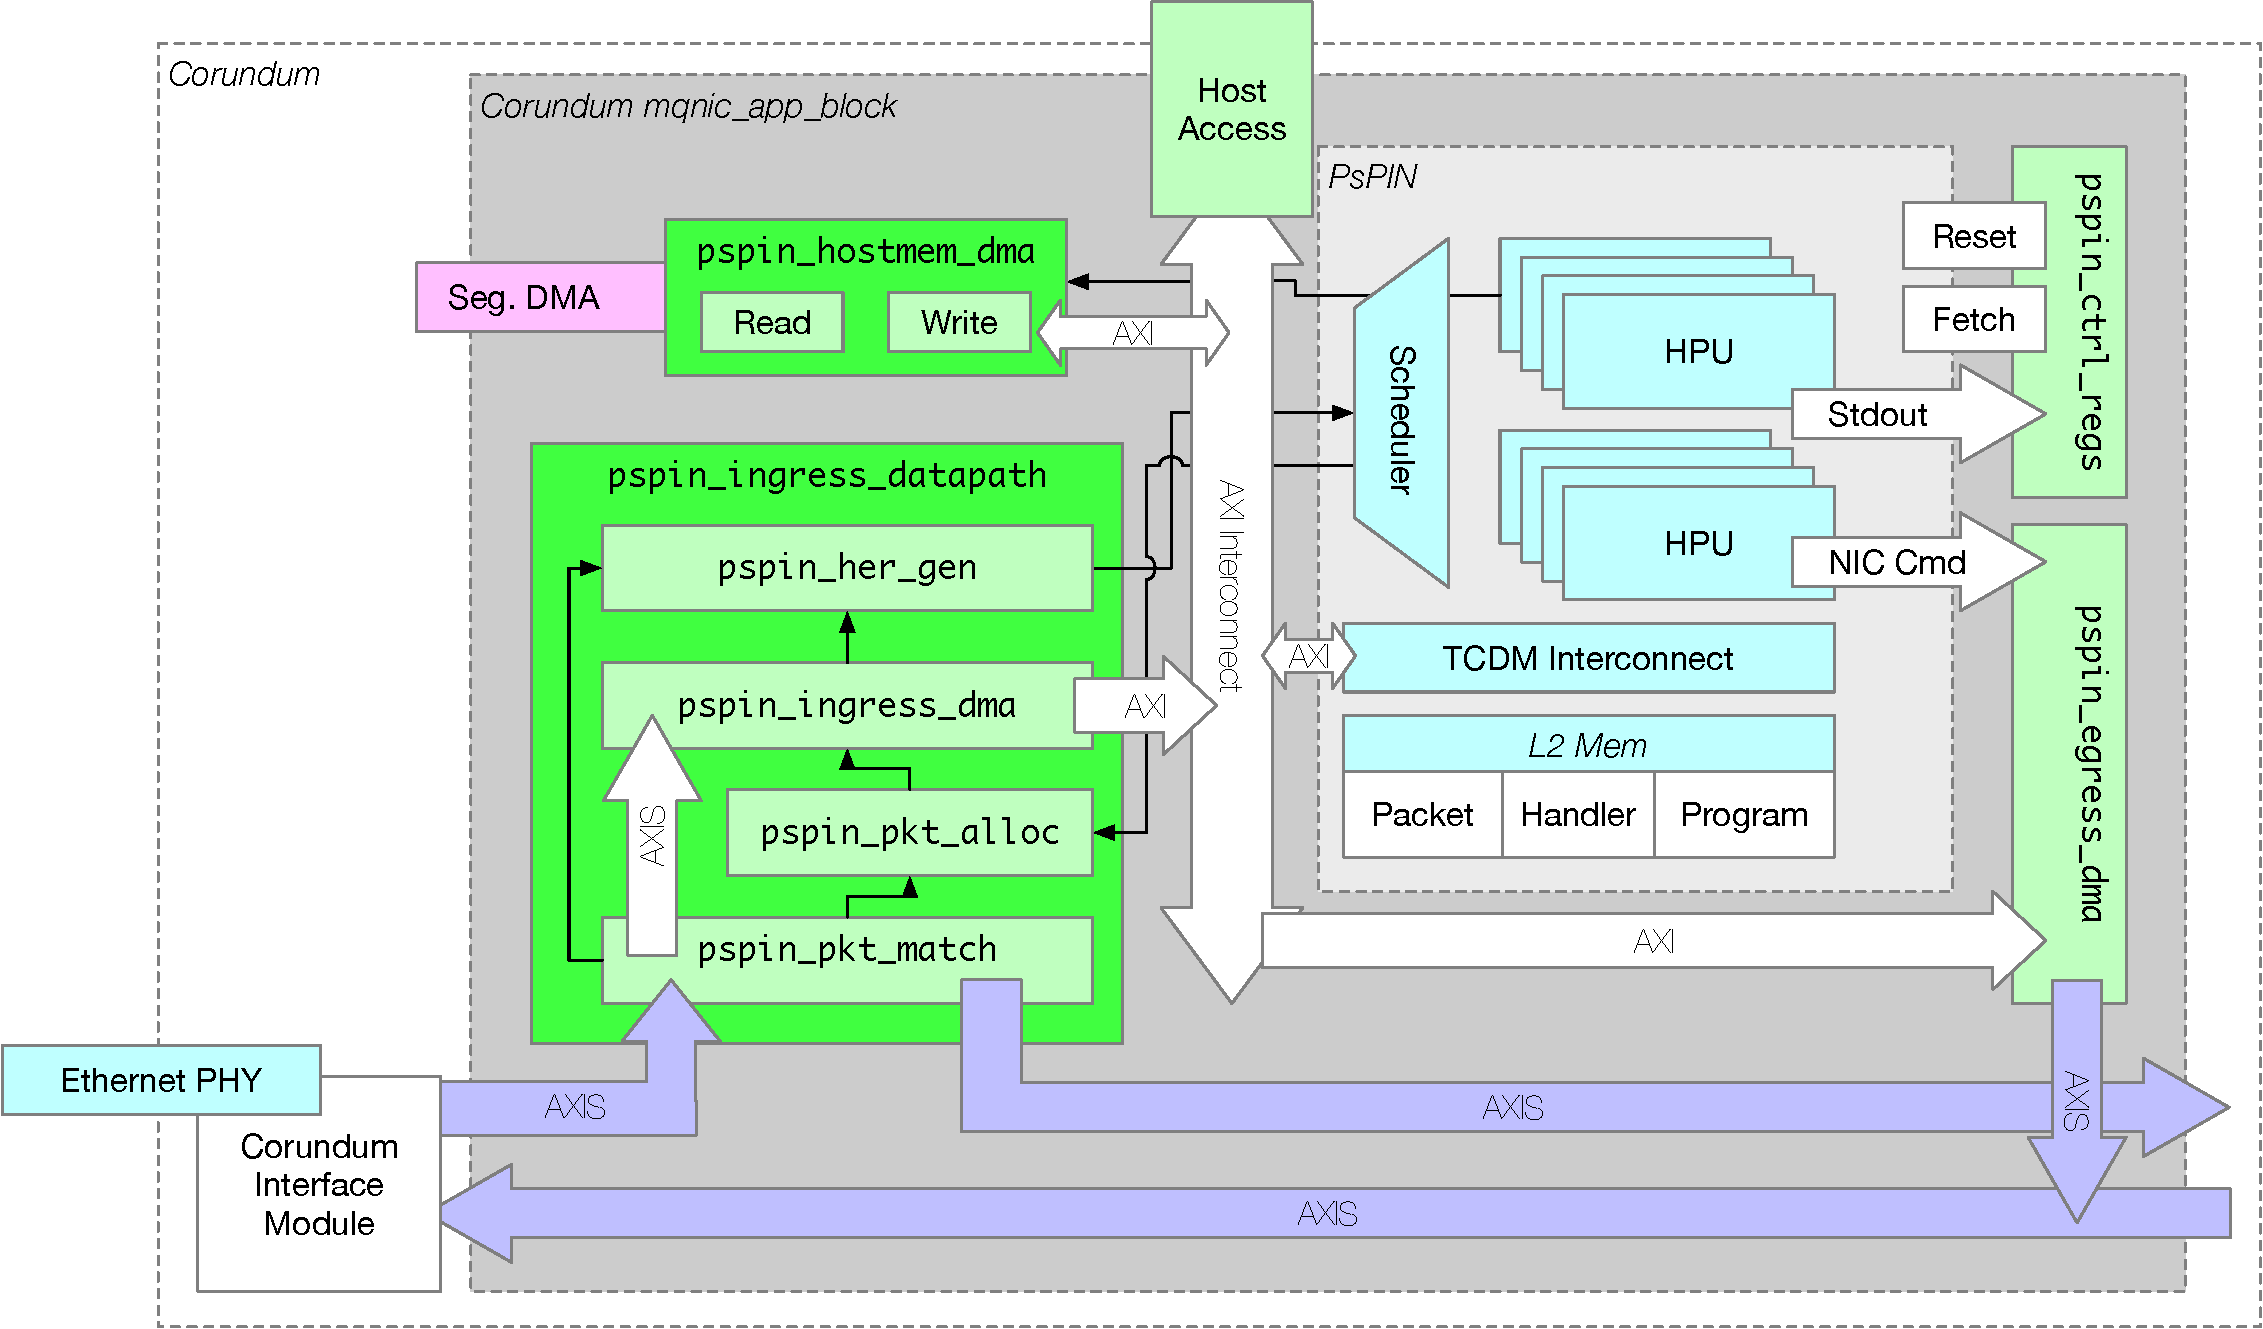
\includegraphics[width=\linewidth]{figures/hw-overview.pdf}
    \caption{Overview of the FPsPIN hardware.  Blocks marked in green are the modules implemented as part of this project to bridge the PsPIN cluster to Corundum.}
    \label{fig:hw-overview}
\end{figure}

\pengcheng{distinguish control path/data path from control flow/data flow of PsPIN discussed in \Cref{sec:background-pspin}.  Brief diagram to highlight which part of the flow we are talking about}

\section{Control path}

The control path handles configuration of the PsPIN cluster as well as the various data path components \emph{before} the actual execution of handler code on the cluster.  There are three important control-path tasks to perform from the host, all of which are implemented over Corundum's slow-path 32-bit AXI-Lite
\timos{what is AXI-Lite? Will this go into Background?}
\pengxu{cross-ref \Cref{sec:fpga-basics}}
interface with an address bus of 16 bits:

\begin{itemize}
    \item to toggle various control registers to the PsPIN cluster and data path components;
    \item to read back standard output produced by PsPIN (i.e., \texttt{printf}); and
    \item to load program code and data onto memory in the PsPIN cluster.
\end{itemize}

\paragraph{Control registers} The control registers are configured through the \texttt{pspin\_\-ctrl\_\-regs} module.  The module exposes an AXI-Lite slave towards the AXI-Lite interconnect and converts this into simple \texttt{valid}-guarded interfaces \timos{what is a valid-guarded interface?} for PsPIN and various data path components to consume.  Some signal groups have requirements on \emph{consistency of update}, that is, the signals in the same group should always be consistent and no partial updates should be visible to the components being controlled.  Checks for this requirement happens in the kernel driver as we will introduce in \Cref{sec:sw-kmod}.  An overview of the exposed control signals from \texttt{pspin\_\-ctrl\_\-regs} is shown in \Cref{tab:ctrl-signals}.

\begin{table}[ht]
    \centering
    \begin{tabular}{lcl}
    \toprule
    Name & Direction & Description \\ \midrule
    \texttt{cl\_fetch\_en} & O & Fetch-enable control to PsPIN \\
    \texttt{aux\_rst} & O & Auxiliary reset for PsPIN and data path \\
    \texttt{cl\_busy} & I & Cluster busy status from PsPIN \\
    \texttt{mpq\_full} & I & MPQ full status bitmap \\
    \texttt{match\_*} & O & Matching engine configuration \\
    \texttt{her\_gen\_*} & O & HER generator configuration \\
    \texttt{stdout\_*} & O & Standard output readback \\
    \bottomrule
    \end{tabular}
    \caption{Overview of the control wires consumed by \texttt{pspin\_ctrl\_regs}.  The configuration for the matching engine, HER generator, and standard output readback are described in the coming sections. \timos{All the names used here do not appear before (HER generator, matching engine) - in Fig 3.1 I see things like pspin\_pkt\_match - so maybe it refers to that, but there should be a piece of text explaining Fig 3.1 which connects those block names to high-level concepts.}}
    \label{tab:ctrl-signals}
\end{table}

The control registers module is designed to allow reconfiguration during normal operation of the system.  Therefore, components that take configuration data from the module are expected to have a explicit \emph{valid} signal, if they expect consistency between multiple registers.  The software that controls these register would then deassert valid, change the registers, and then reassert valid, such that the downstream module can have a consistent configuration.

\paragraph{Standard output access} To facilitate debugging of handler code on the PsPIN cluster, we implement a readback mechanism for the characters printed by the RISC-V cores.  The core executes \texttt{putchar} to write characters into the \texttt{apb\_stdout} module.  Different cores write to separate addresses exported by the module, allowing the module to demultiplex the incoming characters.  The module enqueues the characters toegether with the source core ID in a FIFO.  The FIFO is then read out from \texttt{pspin\_ctrl\_regs}.  To avoid introducing module ports on all levels of RTL hierarchy, we utilise the \emph{hierarchical reference scope}~\cite{noauthor_verilog_nodate} feature of Verilog to connect the output ports from \texttt{apb\_stdout} directly.  Finally, the host can read back the enqueued characters by reading out the \texttt{stdout\_*} registers through the register interface, demultiplex, and store the output as logs for future inspection.

\paragraph{Code and data download} The code and data of the packet handler program on PsPIN need to be loaded into the \emph{program memory} in PsPIN before we can start scheduling packets to execute on the HPUs.  The program memory is accessible through the \emph{host slave} port on the PsPIN cluster.  This port also allows write to the other two memory areas, the \emph{handler memory} and the \emph{packet memory}.  Together, this allows loading of compiled PsPIN program images onto the cluster memory.

We implement such access by connecting the upstream AXI-Lite port from Corundum, through a AXI-Lite interconnect and a AXI-Lite to AXI4 adpater, to the host slave port.  Note that the PsPIN address space on the host slave port is 32-bits.  However, we only have a 24-bit address space from the application block configuration port from Corundum.  Therefore, we perform a \emph{compression} in the address space by mapping the three memory areas closer together into the configuration port address space.  The loader in the userspace library, as later to be described in \Cref{sec:sw-lib}, will encode the PsPIN memory accesses according to this mapping.
\timos{Maybe a picture would be useful here to show the actual mapping?}

\section{Data path}

PsPIN, being a packet processor, needs to have access to the receive and transmit paths in the NIC to function properly.  We introduce in this section the design and implementation of the ingress and egress data path engines that gives PsPIN access to the packet data path.

\paragraph{Attach points of the data path} Corundum provides access to raw Ethernet frames over the AXI Stream interface.  Three attachment points are available to the application block for reading ingress Ethernet frames out, as well as injecting egress frames:

\begin{itemize}
    \item \emph{Direct}: the AXI Stream interface directly after the Ethernet MACs and before most Corundum modules.  The interfaces are synchronous to the MAC clock (322.265625 MHz for 100 Gbps Ethernet).  This offers the lowest possible latency from the application block.
    \item \emph{Sync}: the AXI Stream interface after the CDC (clock domain crossing) FIFO for each port.  These interfaces are synchronous to the Corundum core clock (250 MHz).  They offer comparatively low latency.
    \item \emph{Interface}: the AXI Stream interface after the main packet aggregation FIFO per interface.  These interfaces are per interface (instead of per port; for example a 100 Gbps interface could be split into 4 25 Gbps ports) and are the simplest to process.  They are synchronous to the Corundum core clock (250 MHz).
\end{itemize}

The FPGA board we use, as described in \Cref{sec:fpga-basics} and later in detail in \Cref{sec:eval-setup}, has two 100 Gbps interfaces; each interface can be further split up into 4 25 Gbps ports.  For simplicity of implementation, we attach the PsPIN data path at the \emph{interface} attach point, such that we don't have to multiplex traffic from different ports by ourselves.

\subsection{Ingress}

After a packet has arrived at the \emph{interface} attach point, multiple tasks need to be done for an ingress packet before it lands in PsPIN memory and is ready for processing.  We implement four separate functional blocks as follows; together they form the ingress data path module (\texttt{pspin\_\-ingress\_\-datapath}):

\begin{itemize}
    \item \texttt{pspin\_\-pkt\_\-match}: match if the packet is to be processed by the SmartNIC cluster or to be forwarded to the normal Corundum data path;
    \item \texttt{pspin\_\-pkt\_\-alloc}: allocate buffer for the incoming packet in the L2 packet buffer, free the buffer once it finishes processing;
    \item \texttt{pspin\_\-ingress\_\-dma}: DMA write the packet data into the L2 packet buffer
    \item \texttt{pspin\_\-her\_\-gen}: generate the Handler Execution Request to the PsPIN cluster
\end{itemize}

We explain in detail the design of these modules.  Note that common design considerations presented in \Cref{sec:hw-design-considerations} apply to these modules.

\paragraph{Packet matching engine} \texttt{pspin\_\-pkt\_\-match} exposes one AXI-Stream slave (\texttt{s\_\-axis\_\-nic\_\-*}) towards the upstream packet data that comes from the application block interface in Corundum.  It further exposes two AXI-Stream master ports towards the downstream packet processing logic.  One of them (\texttt{m\_\-axis\_\-pspin\_\-*}) forwards the matched packet data to the rest of the data path components for further processing.  In addition, the module also exposes metadata for the matched packet over a ready-valid interface (\texttt{packet\_\-meta\_\-}) providing the downstream components with the following information:

\begin{itemize}
    \item \emph{Message ID} from the SLMP packet header (see \Cref{sec:slmp} for details of the SLMP protocol), for the \emph{Handler Execution Request} (HER) generator
    \item \emph{EOM (end-of-message) bit} as specified by the matching ruleset, for the HER generator
    \item \emph{Ruleset ID} of the matching ruleset, for the HER generator to select the correct execution context
    \item \emph{Length} of the packet, for the packet buffer allocator
\end{itemize}

Since we need to count the length of the packet, the packet metadata can only be generated after that the packet has been trasferred on the AXI-Stream interface.  A later stage in the data path (the ingress DMA engine) will reverse this dependency by buffering the packet data.

We adopt a simple approach to define the matching rules similar to the IPTables U32 match~\cite{cohen_iptables_nodate}.  The matching engine provides a configurable number of \emph{rulesets}.  We expose ruleset configuration to the host as control registers.  Each ruleset is defined by a configurable number of \emph{matching rules} for the \emph{matching units}, which, each one on its own, matches against a 32-bit word of the packet and produces a boolean output.  Given index $I$, 32-bit mask $M$, 32-bit start value $S$, and 32-bit end value $E$, the matching unit output is defined as:

\[
\text{Output} := S \le (\text{Packet}[4I:4I+3] \mathbin{\&} M) \le E
\]

Each ruleset defines a \emph{mode} in which the output from the matching units are combined into the match output of the ruleset.  We currently implement two modes: \texttt{MATCH\_\-AND}, which combines the match unit outputs with a logical AND; and \texttt{MATCH\_\-OR}, for a logical OR.  The module is designed such that it is easy to add another combination mode, if such a use case rises (for example an \emph{exactly-one} combination mode).  If any of the installed rulesets matched on the packet, the module marks the packet as matched for further processing in the data path.  The module then sets the \emph{ruleset ID} metadata of the packet accordingly for execution context selection as described later when we introduce the HER generator.
\timos{Nice explanation, maybe add an example?}

The other AXI-Stream master interface (\texttt{m\_\-axis\_\-nic\_\-*}) performs a \emph{pass-through} of packets that did not match with any installed rulesets back into the regular Corundum packet data path.  This allows the NIC with PsPIN attached to it to still function as a normal NIC when PsPIN is not configured.  It also enables host processing of traffic that is not of interest to PsPIN, for example in handling the \emph{Address Resolution Protocol} (ARP) as described in \Cref{sec:l3-protocol-handling}, or when implementing an application-level control plane in the MPI Datatypes application as described in \Cref{sec:mpi-datatypes-demo}.

\pengcheng{clarify that FPsPIN is a blend of on-path and off-path}

\paragraph{Packet buffer allocator} The packet buffer allocator takes the metadata from the matching engine and allocates a buffer for the packet in the L2 packet buffer of PsPIN.  It runs the allocation algorithm based on the packet length, adds the resulting address of the allocated buffer to the packet metadata, and forwards the metadata to the DMA engine to actually write the packet into the memory.  It takes in the \emph{feedback} from PsPIN, which denotes that a packet has been processed and its buffer can be freed, to free the buffer correctly.  It further outputs one statistics counter of how many packets have been dropped due to the buffer being full.

The Verilator model originally developed in the PsPIN project uses a software-based ring buffer in the simulation testbench to allocate space for incoming packets in the packet buffer.  The free algorithm needs to keep a queue of out-of-order frees and is thus difficult to implement in hardware.  However, most packets on the Internet and in data center environments follow a \emph{bimodal} distribution in size: 40\% of packets are below 64 bytes and another 40\% are 1500 bytes (the MTU of an Ethernet/IP network)~\cite{john_analysis_2007,benson_understanding_2009}.  We thus take a simpler \emph{fixed-size} allocation approach: we partition the packet buffer into two halves; in one half we make fixed 64-byte slots, and in the other half we make 1536-byte slots.  We store these free slots in two separate FIFOs.  We then handle allocation and free simply by popping from and pushing to the respective FIFOs.  This way, we greatly simplify the hardware implementation of the allocator while not sacrificing too much buffer utilisation on internal fragmentation.

\pengcheng{(how) do we claim against fragmentation?  should we state that we can just increase the size of the packet buffer?}
\timos{Do we care? We can simply say we also partition the packet buffer in two regions, one for small and one for large packets, then there is no fragmentation problem. If you mean internal fragmentation (an allocated packet might not always be fully used) ignore it.}

\paragraph{Ingress DMA} The ingress DMA module takes the allocated address and length in the packet metadata and performs a DMA transaction to write the packet data to the PsPIN NIC inbound memory port.  Upon finish of the DMA request, the module forwards the packet metadata on to the HER generator in the data path, such that the packet can get scheduled on the PsPIN cluster.  We use the \texttt{axi\_\-dma\_\-wr} module from the Corundum AXI IP library to perform the actual DMA operation.

One complication to be handled in this module is that the matching engine could only generate the packet metadata \emph{after} transferring the packet data on the AXI-Stream bus.  This is due to a dependency introduced by needing to count the length of the message.  This is handled by introducing a shallow \texttt{axis\_\-fifo} to reverse this dependency for the DMA module.

\paragraph{HER generator} Once the packet is written to the right place in the L2 packet buffer of PsPIN, the data path can now schedule the packet for processing by issuing a \emph{Handler Execution Request} (HER) to PsPIN.  Part of the information required to generate a HER comes from the packet metadata, such as the message ID and if the packet is the last in a message (\emph{End-Of-Message}, EOM).  The rest of the HER stores the address of the handler functions that the packet should be processed with, as well as the host DMA and L2 memory regions.  We expose a register control interface to the host through \texttt{pspin\_\-ctrl\_\-regs}.

\paragraph{Collective ingress data path} \texttt{pspin\_\-ingress\_\-datapath} does not provide extra logic by itself, as it is simply an instantiation wrapper of the four data path components.  It keeps the parameters in synchronisation among the data path modules and allows for one single place to pass in custom parameters.  It also functions as a top module for end-to-end simulation and unit tests so that we can validate that the data path modules have consistent assumptions of how each other operates.
 
\subsection{Egress}

PsPIN also needs the ability to send packets into the network.  This is needed to either complete a protocol by sending back acknowledgements, or transmit packets to other nodes e.g.\ to implement in-network AllReduce~\cite{de_sensi_flare_2021} with PsPIN.  The transmission of the prepared egress packet is handled by \texttt{pspin\_\-egress\_\-datapath}; we discuss about potential problems in preparing the outgoing packet and solutions in \Cref{sec:l3-protocol-handling}.

\texttt{pspin\_\-egress\_\-datapath} handles egress commands from PsPIN.  With the Corundum IP \texttt{axi\_\-dma\_\-rd}, the module performs a DMA read from the packet buffer and gets an AXI-Stream bus that contains packet data.  It then injects the AXI-Stream into the outbound AXI Stream of Corundum with an AXI-Stream arbiter (\texttt{axis\_arb\_mux}).  The arbiter is wired such that the outgoing traffic from PsPIN has priority over egress traffic from the host for maximum possible throughput from PsPIN.  It can also be configured to use round-robin arbitration to ensure fairness between the host and PsPIN on outgoing packets.

\pengcheng{In FPsPIN, PsPIN does not interface with the ``command unit'' of Corundum, since injecting packets do not require explicit commands.   This way we do not take advantage of checksum offloading, timestamping, etc.  We need to figure out how to do this (resembling the host driver); cross-ref future work}

\section{Host DMA}

A feature that distinguishes the sPIN programming model from other packet processing paradigms intended for intrusion detection (IDS), for example \cite{khazraee_rosebud_2023}, is the ability of packet handlers to read from and write to host memory.  Between PsPIN and Corundum, this is enabled through the \texttt{pspin\_hostmem\_dma} module.  The module bridges the AXI master port of the PsPIN cluster to the segmented DMA interface of Corundum~\cite{forencich_verilog_2023}, which takes a RAM port and a separate command bus.  We utilize the AXI-Stream DMA client (\texttt{dma\_\-client\_\-axis\_\-source}, \texttt{dma\_\-client\_\-axis\_\-sink}) from Corundum to convert the output AXI Stream bus to AXI4 channels.  For write requests from PsPIN, the module first issues a DMA command to the AXI-Stream client to capture the write data in a dual-port RAM buffer (\texttt{dma\_\-psdpram}); it then issues a command to the Corundum DMA subsystem to DMA the data from the buffer RAM to the host memory.  The read process happens in the reverse order.

There are some notable limitations in this approach, namely that the adapter is not fully AXI-compliant in multiple corner cases.  We do not support irregular bursts (narrow bursts or modes other than \texttt{INCR}), as well as interleaved read requests.  Unlike AXI4, the PCIe interface also does not support arbitrary \emph{byte enable} (BE) configurations, so we also do not support these cases.  While it is theoretically possible to handle all these corner cases, it would lead to very long combinatorial paths of the resulting hardware, which would then take too much engineering effort to fix.  However, these limitations are acceptable in our use case, since the DMA bus master in PsPIN does not issue such requests.

One important corner case to implement correctly, however, is \emph{unaligned writes}.  As mandated by the sPIN specification and also as we later will see in \Cref{sec:mpi-datatypes-demo}, unaligned transfers are essential to some applications.  While it is possible to implement unaligned transfers in software by reading the affected word first to compose and issue an aligned transfer, the extra memory read transactions (up to \emph{two} extra reads for one unaligned write) would significantly hurt performance.  Fortunately, the Corundum DMA subsystem fully supports unaligned transfers.  As AXI4 expresses unaligned writes as aligned writes with strobe (byte-enable), we implement an \emph{address recovery} procedure that calculates the original address and length from the AXI burst strobe (\texttt{WSTRB}) signal of the first and last beat in the AXI transaction.  The module then issues the unaligned transfer to the client and Corundum DMA subsystem as normal.

\section{Design considerations} \label{sec:hw-design-considerations}

As we stated in \Cref{sec:contributions}, it is not a goal of this thesis project to achieve the absolute highest possible performance.  The hardware implementations are thus designed with the approach of the \emph{simplest} hardware implementation possible.  This means that modules with complicated logic e.g.\ the host DMA engine are simple state machines without pipelining.  We also do not support concurrent requests, even if the protocol supports it (in the case of AXI4 on the host DMA engine).  For the purpose of a full-system demo, we argue later in \Cref{sec:hw-analysis} that these design limitations would not impact the overall system performance.

Another limitation of the hardware performance is in the PsPIN implementation.  PsPIN uses the PULP~\cite{rossi_pulp_2015} RISC-V cores and AXI infrastructure, which are originally designed for ultra-low-power ASIC platforms.  This means that they are optimised for recent ASIC process nodes and thus have long critical paths, making them not suitable for FPGA operation.  While some parameter tweaking allowed us to break very long critical paths e.g.\ single cycle bus across the entire SoC, most components need to be redesigned to reach a higher $F_{\text{max}}$ on FPGAs.  We discuss possible directions to a solution in \Cref{sec:improving-fmax}.

The lengthy critical paths of PULP and thus PsPIN on FPGAs mean that without significant re-engineering, the packet processing cluster could only run at a lower frequency.  This situation is further worsened by the area requirements of the original PsPIN design: the 4-cluster configuration that was used in the original PsPIN paper proved to be extremely difficult, if possible at all, to place and route on the FPGA device we are using.  We thus use a 2-cluster configuration with reduced memory sizes.  To further resolve the routing congestion problems, we employ the incremental implementation flow provided by Xilinx as described in \Cref{sec:eval-setup}.

In contrary to PsPIN, Corundum runs at 250 MHz on the target Xilinx devices.  While it is possible to retarget Corundum to run at a lower frequeny, we would to have to reconfigure the clock domains and validate that the resulting design still works properly; this is a non-trivial process.  Instead, we opted to \emph{only} run the PsPIN cluster and the closely coupled data path engines at a lower frequency (40 MHz for the evaluation in this thesis; more about the setup in \Cref{sec:eval-setup}).  We perform \emph{clock-domain crossing} (CDC) on the AXI-Lite and AXI-Stream interfaces with standard IP blocks from Xilinx.  We isolate timing optimisation as a separate task and keep it out of the scope this thesis due to time constraints of the project.

\chapter{Software}

Three classes of software are required for the full operation of FPsPIN: kernel modules, user-space library, and utilities.  An overview of the software landscape on the CPU can be seen in \Cref{fig:sw-overview}.

\begin{figure}
    \centering
    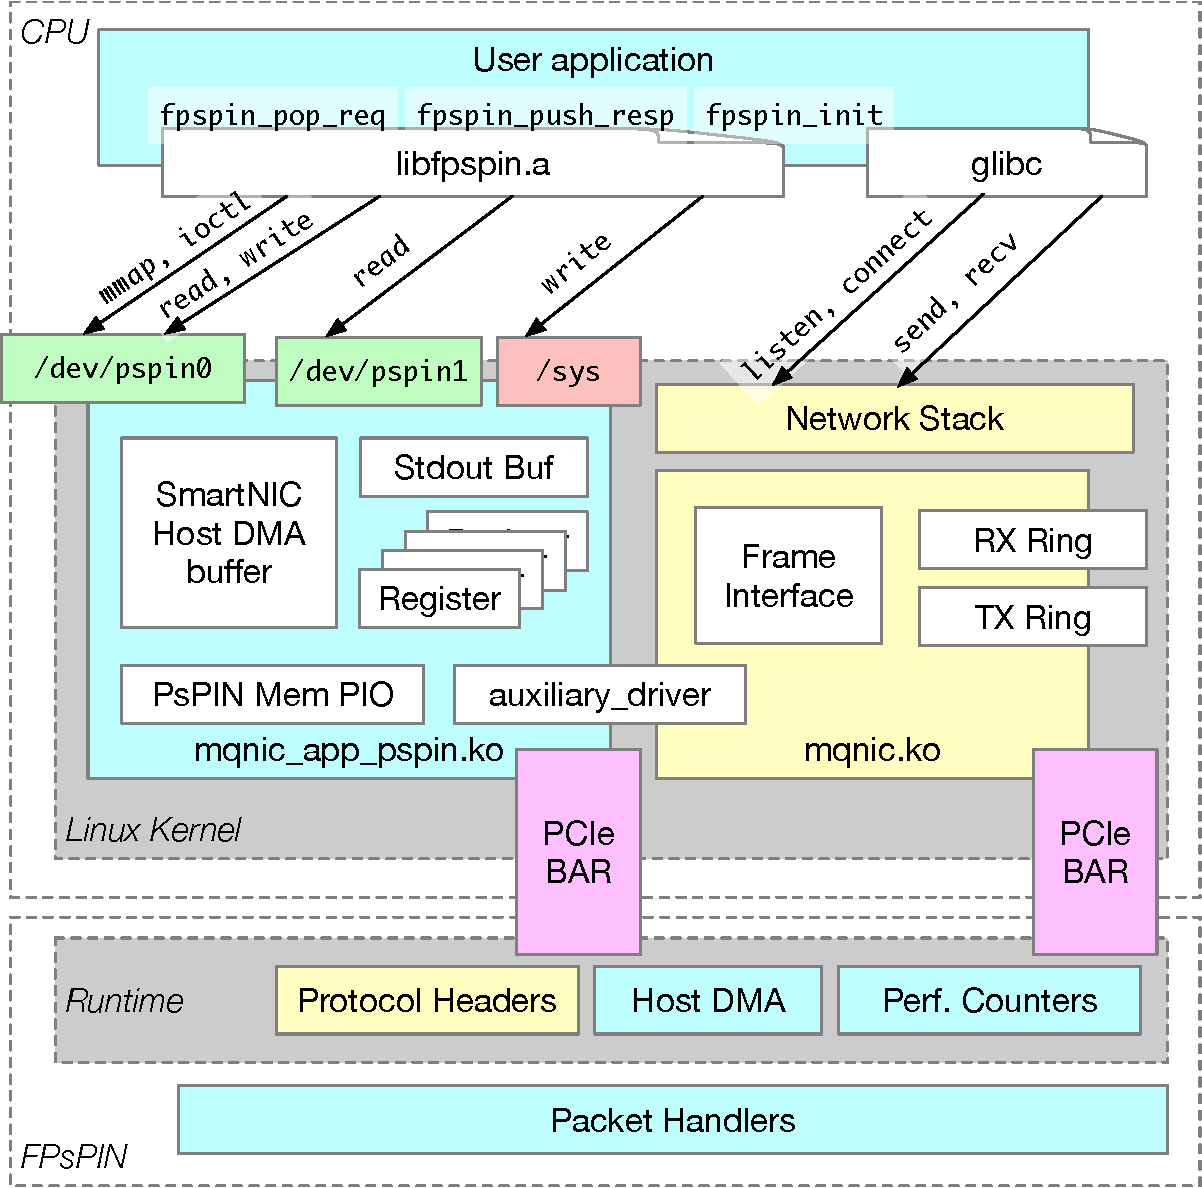
\includegraphics[width=\linewidth]{figures/sw-overview.pdf}
    \caption{Overview of the software on the host.  Yellow blocks denote existing software, while blue boxes show software developed in this project's scope.  Note that we use only standard Unix syscalls (\texttt{read}, \texttt{write}, \texttt{mmap}, \texttt{ioctl}) between the user and kernel space.}
    \label{fig:sw-overview}
\end{figure}

\section{Kernel modules} \label{sec:sw-kmod}

Two kernel modules are required for the full functionality.  \texttt{mqnic.ko} is unmodified from Corundum and provides basic functionalities of the FPGA device as an Ethernet NIC, that is, packet send and receive.  On top of this, \texttt{mqnic\_app\_pspin.ko} communicates with the Corundum module over the auxiliary bus facility in the Linux kernel, providing low-level register access into the cluster and data path and management of host DMA buffers.  The application block module exposes two device nodes (\texttt{/dev/pspin\{0,1\}}) and a selection of device registers over \texttt{sysfs}.

\section{User-space library} \label{sec:sw-lib}

The userspace library \texttt{libfpspin.a} wraps around the device files and \texttt{sysfs} properties to several C APIs to be called by the host part of an sPIN application.  \Cref{tab:user-apis} shows a list of different operations to be performed by the host application.  A typical host application will have a thread that polls for incoming requests from the cluster to handle.  In addition, the traditional Unix networking model through \texttt{libc} is still available.

\begin{table*}[!t]
    \centering
    \begin{tabular}{ll}
    \toprule
    Functions & Description \\ \midrule
    \texttt{fpspin\_ruleset\_*} & Configure the matching engine for custom matching rules (UDP packets, etc.) \\
    \texttt{fpspin\_\{init,exit\}} & Initialise and cleanup of FPsPIN context; loads code onto the cluster \\
    \texttt{fpspin\_\{pop\_req,push\_resp\}} & Respond to host requests from the smart NIC \\
    \texttt{fpspin\_get\_avg\_cycles} & Obtain telemetry data from handler execution \\
    \bottomrule
    \end{tabular}
    \caption{API functions for the heavy-lifting to the basic interface from the kernel modules.  These functions are provided by \texttt{libfpspin.a}.}
    \label{tab:user-apis}
\end{table*}

\paragraph{Utilities} Two scripts help the operation of FPsPIN. \texttt{cat\_stdout.py} reads the standard output from the cluster onto the host, sorts them into different files per core, and stores the result in files for a later review.  The \texttt{setup-netns.sh} script assigns the test and tester network interfaces to the separate network namespaces for ease of evaluation.

\chapter{sPIN Revisited} \label{chap:spin-revisited}
\begin{chapquote}{John Drury Clark, \textit{Ignition!--An Informal History of Liquid Rocket Propellants}}
Their guess turned out to be right, but one is reminded of E. T. Bell's remark that the great vice of the Greeks was not sodomy but extrapolation.
\end{chapquote}

Throughout the process of building the FPsPIN demo, we ...
\pengcheng{intro: missing parts in the sPIN specification for real-world operation.  Communicated back to the sPIN team and some are already adopted into the current sPIN specification}

\section{Handler Initialisation} \label{sec:handler-init}
\pengcheng{How to initialise handler states?  device function that's called once, that is not a handler (no HER meta etc.)}
\pengcheng{Init with host involvement.  Should be defined in sPIN as extended\_init or something}

\section{Streaming Host DMA} \label{sec:streaming-host-dma}
\pengcheng{we currently have one large host DMA region per execution context.  it may be beneficial if we stream host processing by having the app call mmap multiple times to feed a ring buffer in the kernel/hardware to feed to the HER generator so that we have one buffer per message.  How to formalise this in sPIN?}

\section{Packet Matching Rules}

\section{Network-layer Protocol Handling} \label{sec:l3-protocol-handling}
\pengxu{for example incoming ARP probes when using Ethernet/IP}
\pengxu{Sending packet: share neighbour buffer with host?  Implement ARP stack in sPIN?}

\section{Messaging and Reliability Layer: SLMP} \label{sec:slmp}
\pengxu{protocol should be message oriented (instead of TCP).  reliability requirements: SCTP, DCCP, SLMP, pure UDP}
\pengxu{SLMP ACK configuration}

\section{Scheduler Concurrency Control}
\pengxu{Ability to control degree of parallelism \& locality.  Possible implementation: core mask on the scheduler}

\section{Support for Diverse Memory Architectures}
\pengxu{Corundum supports NIC-attached DDR or HBM; should extend the }
\chapter{Evaluation}

We present the preliminary evaluation results of the FPsPIN implementation.  We have two results presented here: \emph{theoretical} analysis of latencies of various fast-path components and \emph{end-to-end} latency measurements on real hardware for two demo applications.
%Please keep in mind that the project at this point is still ongoing; there is still plenty of room for optimization due to the design and implementation decisions made under the time constraints.
% \misha{I would remove the sentence: "Please keep in mind that the project at this point is still ongoing; there is still plenty...", since we already mentioned the state of the project in the intro.}

\section{Experiment Setup} \label{sec:eval-setup}

The experiments are done on the AMD server with the Ryzen 7 2700 CPU and the PCIe-attached Xilinx VCU1525\footnote{\url{https://www.xilinx.com/products/boards-and-kits/vcu1525-a.html}} development kit.  The two 100 Gbps QSFP Ethernet ports on the FPGA board are attached via one Direct-Attached-Copper (DAC) cable.  A diagram of the experiment platform is shown in \Cref{fig:experiment-setup}.  We use Ubuntu 20.04.4 LTS with Linux 5.15.0-71-generic, Vivado 2020.2, and the PULP RISC-V toolchain\footnote{\url{https://github.com/pulp-platform/pulp-riscv-gnu-toolchain}}. 
%\misha{probably we want to mention the bandwidth of the ethernet ports.}

On the FPGA, Corundum runs at its native frequency of 250 MHz.  Due to PsPIN IP not being designed for FPGAs but for ASICs, the PULP RISC-V cores have long critical paths.  As a result, the processing cluster runs at 40 MHz.

\begin{figure}
    \centering
    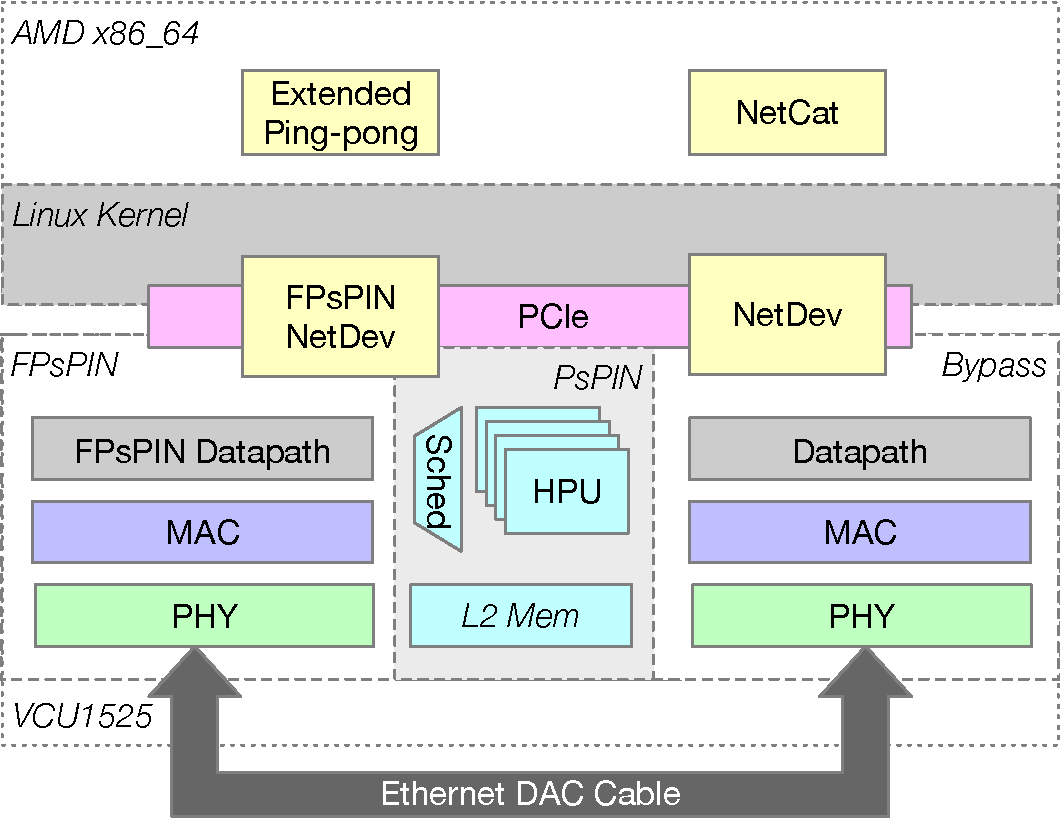
\includegraphics[width=.9\linewidth]{figures/experiment-setup.pdf}
    \caption{The experiment setup.  The host application of sPIN and the tester (\texttt{netcat} in the diagram) are in two separate network namespaces to prevent the direct loopback mechanism in Linux.}
    \label{fig:experiment-setup}
\end{figure}

\subsection{Theoretical data path analysis} \label{sec:hw-latency-analysis}

We estimate the latency of the hardware components as described in \Cref{sec:hw}.  \Cref{tab:lat-cycles} shows the latency in cycles based on the state machine construction in the Verilog RTL code, the frequency, and the latency time in nanoseconds.  Due to a limitation in the implementation, not all modules have a constant latency (\texttt{pspin\_ingress\_dma}), but is instead linearly related to the packet size.  We show in the next paragraph that these latency numbers are negligible compared to other parts of the system and, thus, would not have a big impact on overall latency.

\begin{table}[!htbp]
    \centering
    \begin{tabular}{lccc}
    \toprule
    Module & Cycles & Frequency (MHz) & Latency (ns) \\ \midrule
    Matching engine & 4 & 40 & 100 \\
    Allocator & 0 & 40 & 0 \\
    Ingress DMA & 8\mytilde{}70 & 40 & 200\mytilde{}1750 \\
    HER generator & 0 & 40 & 0 \\
    Host DMA & \emph{n/a} & 250 & \mytilde{}450 \\
    \bottomrule
    \end{tabular}
    \caption{Latency estimation for various data path modules in cycles and nanoseconds.  Note that as the host DMA goes over PCIe to the host DRAM, the exact latency in cycles is difficult to estimate; the latency in nanoseconds is measured on real hardware via the Integrated Logical Analyzer (ILA) on Xilinx platforms.}
    \label{tab:lat-cycles}
\end{table}

\subsection{Demo applications on real hardware}
We present two end-to-end demo applications to showcase that FPsPIN has realistic performance characteristics. We show that it is possible to write arbitrary packet-processing applications for the platform. The two applications follow the same operation workflow, also shown in \Cref{fig:demo-apps}:

\begin{enumerate}
    \item a packet comes in and matches for SmartNIC processing
    \item the cluster processes the packet
    \item (optionally), the cluster forwards it to the host for further processing
    \item the cluster sends back a response packet
\end{enumerate}

\begin{figure}
    \centering
    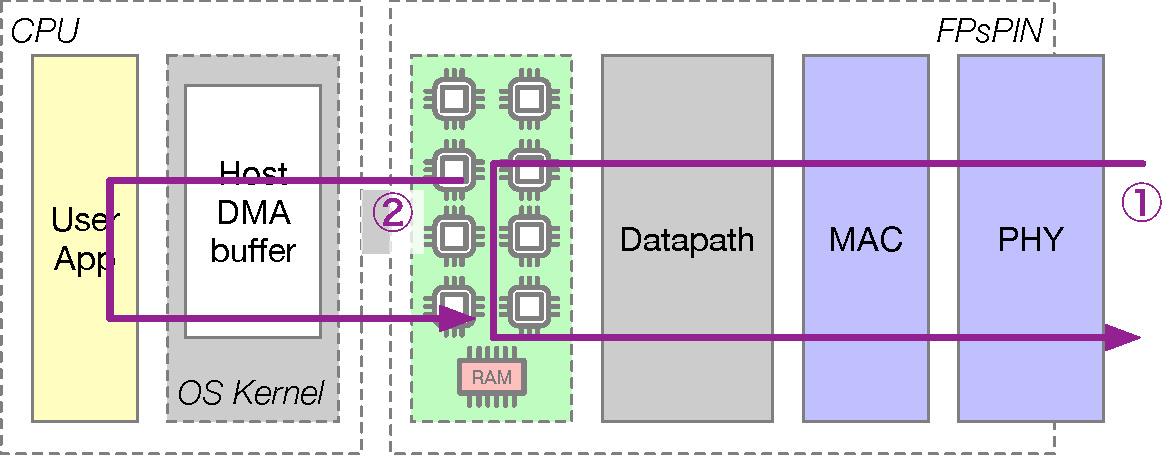
\includegraphics[width=.9\linewidth]{figures/demo-apps.pdf}
    \caption{Workflow of the demo applications.  The cluster can forward the packet to the host application for further processing, denoted with the red dashed arrow.}
    \label{fig:demo-apps}
\end{figure}

\paragraph{ICMP Echo ("ping")}  We evaluate the end-to-end system latency with the ICMP-Echo-Response test, also known as the \emph{ping} test.  For an ICMP payload size of 56 (the default value) and 1400 bytes, we evaluate two different scenarios:

\begin{itemize}
    \item Without host: the handler code swaps the IP address and Ethernet address of the incoming packet, sets the reply bit of the ICMP Echo packet and recalculates the ICMP checksum.
    \item With host: same as above, but the ICMP checksum calculation is performed on the host.
\end{itemize}

The resulting latency measurement is shown in \Cref{tab:icmp-ping}.  We notice that for small packets (56 B payload), FPsPIN shows performance on par with the host-only scenario; a further breakdown shows that half of the 33 us latency comes from the handler execution.  As explained in \Cref{sec:future-work}, one of the future works planned is to increase the $F_{\text{max}}$ of the design.  The projected latency of PsPIN, either with or without host processing, is then significantly better than the host-only case.

Another important purpose of SmartNICs is an offloading -- freeing precious CPU cycles from networking tasks.  Even though we notice slightly worse E2E latency for larger payloads, the on par results combined with the fact that the CPU can stay completely out of the reply processing and do other useful work.  This makes a compelling case for high-bandwidth scenarios to use FPsPIN for offloading communication tasks.

\begin{table}[!ht]
    \centering
    \begin{tabular}{clccc}
    \toprule
    Size (B) & Setup & E2E (us) & Handler (us) & Proj. E2E (us) \\ \midrule
    56 & H & \textbf{29} & \emph{n/a} & \emph{n/a} \\
    56 & P & 33 & 17 & {\color{acmgreen}\textbf{18}} \\
    56 & P+H & 37 & 21 & {\color{acmgreen}\textbf{19}} \\ \midrule
    1400 & H & \textbf{33} & \emph{n/a} & \emph{n/a} \\
    1400 & P & 264 & 244 & {\color{acmyellow}\textbf{59}} \\
    1400 & P+H & 124 & 104 & {\color{acmyellow}\textbf{36}}\\
    \bottomrule
    \end{tabular}
    \caption{Latency measurements of the ICMP ping handler under different operating scenarios: H denotes the baseline case (normal NIC, no PsPIN intervention; marked in bold); P denotes PsPIN-only; P+H denotes PsPIN and host together.  The size column denotes the ICMP payload size (\texttt{-s} argument in \texttt{ping(8)}).  The handler latency correspond to PsPIN running at 40 MHz.  The projected end-to-end latency scales the handler latency to 250 MHz, assuming the rest of the latency stays fixed.}
    \label{tab:icmp-ping}
\end{table}

\paragraph{UDP ping-pong} While the ICMP ping protocol allows good performance characterisations of FPsPIN, the demo application does not showcase what FPsPIN is capable of, due to the rigidity of the protocol: it mandates that the response payload must stay the same as the request.  The UDP ping-pong demo allows more flexibility by allowing the responder to send back arbitrary data.  We use OpenBSD \texttt{netcat} to start a UDP connection.  The packet handler in FPsPIN manipulates the payload by \emph{appending} an upper-case version of the payload to the old payload, recalculating necessary lengths and checksums, and sending the packet back.

\Cref{tab:udp-ping} shows the latency measurements of the UDP ping-pong demo.  We notice that the handler execution time aligns with that of ICMP ping in the case with host processing (18 us); the PsPIN-only setup showed even lower handler latency (5 us) due to UDP not requiring a payload checksum.  However, the end-to-end latency in the order of milliseconds show that the tester-side UDP stack added a significant amount of latency and measuring variance.  Nevertheless, the demo is still useful in demonstrating the capabilities of a PsPIN handler.

\begin{table}[!h]
    \centering
    \begin{tabular}{lcc}
    \toprule
    Setup & E2E (ms) & Handler (ms) \\ \midrule
    P & 5.1 & 0.005 \\
    P+H & 5.7 & 0.018 \\
    \bottomrule
    \end{tabular}
    \caption{Latency measurements of the UDP ping-pong handler.  We only measure PsPIN and PsPIN+Host setups due to a lack of an existing UDP ping-pong responder.}
    \label{tab:udp-ping}
\end{table}

\chapter{Future Work}

\paragraph{Throughput evaluation} We performed extensive latency characterisation of FPsPIN in \Cref{sec:eval}.  However, a thorough throughput analysis would help further identify bottlenecks and limitations in the implementation.  We plan to test the theoretical throughput of PsPIN handlers with synthetic benchmarks, as well as real-world applications, both with and without host processing.

\paragraph{Improving $F_{\text{max}}$} An important factor in the current FPsPIN E2E latency as shown in the ICMP ping demo is the handler processing latency.  This is due to the PULP cluster being designed for ASIC and not optimised for maximum $F_{\text{max}}$ on FPGAs.  We plan to integrate higher frequency RISC-V cores designed FPGA, for example VexRiscv\footnote{\url{https://github.com/SpinalHDL/VexRiscv}}, as well as optimise critical paths in the design, to further lower this latency.

\pengcheng{Explore possible timing relaxations such as increasing the SRAM latency}

\paragraph{Real-world applications} We showcased the capabilities of PsPIN handlers through the UDP ping-pong demo.  However, it would be more beneficial to have real-world applications instead of synthetic benchmarks only.  To further explore in this aspect, we are implementing a memcached-style offloaded key-value store application.  We are also working on porting the MPI Datatypes handlers~\cite{Di_Girolamo_2019} to the FPsPIN platform.

\paragraph{Multi-tenancy} Tenant oversubscription is a typical approach to improve NIC resource utilization in a virtualized data center environment. We aim to enable fair scheduling mechanisms both in hardware and software in the next iterations of the FPsPIN design.

\chapter{Conclusion}
\begin{chapquote}{Lewis Carroll, \textit{Alice's Adventures in Wonderland}}
``Begin at the beginning, '' the King said, very gravely, ``and go on till you come to the end: then stop.''
\end{chapquote}

We set out to build FP\acs{spin} as a faster evaluation platform for \ac{spin} handlers that could run the handlers faster than the cycle-accurate simulation from P\acs{spin} and provide a more complete programming model with host applications.  We presented the detailed design and implementation of the hardware (\Cref{chap:hardware}) and software (\Cref{chap:software}) components of the system.  The successful implementation and evaluation of the ping-pong, \ac{mpi} datatypes, and \ac{slmp} file transfer benchmarks (\Cref{chap:eval}) shows that this goal has been sufficiently reached with FP\acs{spin}.

Another important goal of building FP\acs{spin} is to contribute insights and feedback from actually building a \ac{spin} \ac{nic} back to the \ac{spin} specification.  We identified diverse potential improvements, including reliability protocols, telemetry requirements, scheduler improvements, and many more (\Cref{chap:spin-revisited}).  We believe that our feedback would help \ac{spin} become more comprehensive and realistic in achieving its vision for in-network-computing.

Our comprehensive evaluation of FPsPIN through the three benchmarks systematically characterised its performance in latency, throughput, and computation/communication overlap.  We showed that FPsPIN achieved stable latency advantage against the baseline host-only case in the ping-pong demo (\Cref{sec:demos-ping-pong}) and near-perfect overlap in the \ac{mpi} datatypes demo (\Cref{sec:mpi-datatypes-demo}).  We also showed that the real-world throughput of FPsPIN in the \ac{mpi} datatypes benchmark leaves much to be expected compared to the baseline speed test and synthetic \ac{slmp} file transfer demo (\Cref{sec:slmp-demo}), largely due to the low performance of the measly \ac{pulp} cores currently used by FP\acs{spin}.

This shortcoming in throughput provides an outlook of possible improvements to FP\acs{spin} through the integration of a better \ac{hpu} core designed for \ac{fpga}s (\Cref{sec:improving-fmax}).  Even more interestingly, it opens up possible future research in \ac{hpu} architecture on domain-specific acceleration in packet processing (\Cref{sec:hpu-arch}).  We are excited to see future progress in this domain.


\appendix

\chapter{Appendix}

You can defer lengthy calculations that would otherwise only interrupt
the flow of your thesis to an appendix.


\backmatter

\bibliographystyle{IEEEtran}
\bibliography{IEEEabrv,zotero}

\chapter{Acronyms}

\begin{flushleft}
    \begin{footnotesize}
        \begin{multicols}{2}
            \printacronyms[heading=none]
        \end{multicols}
    \end{footnotesize}
\end{flushleft}

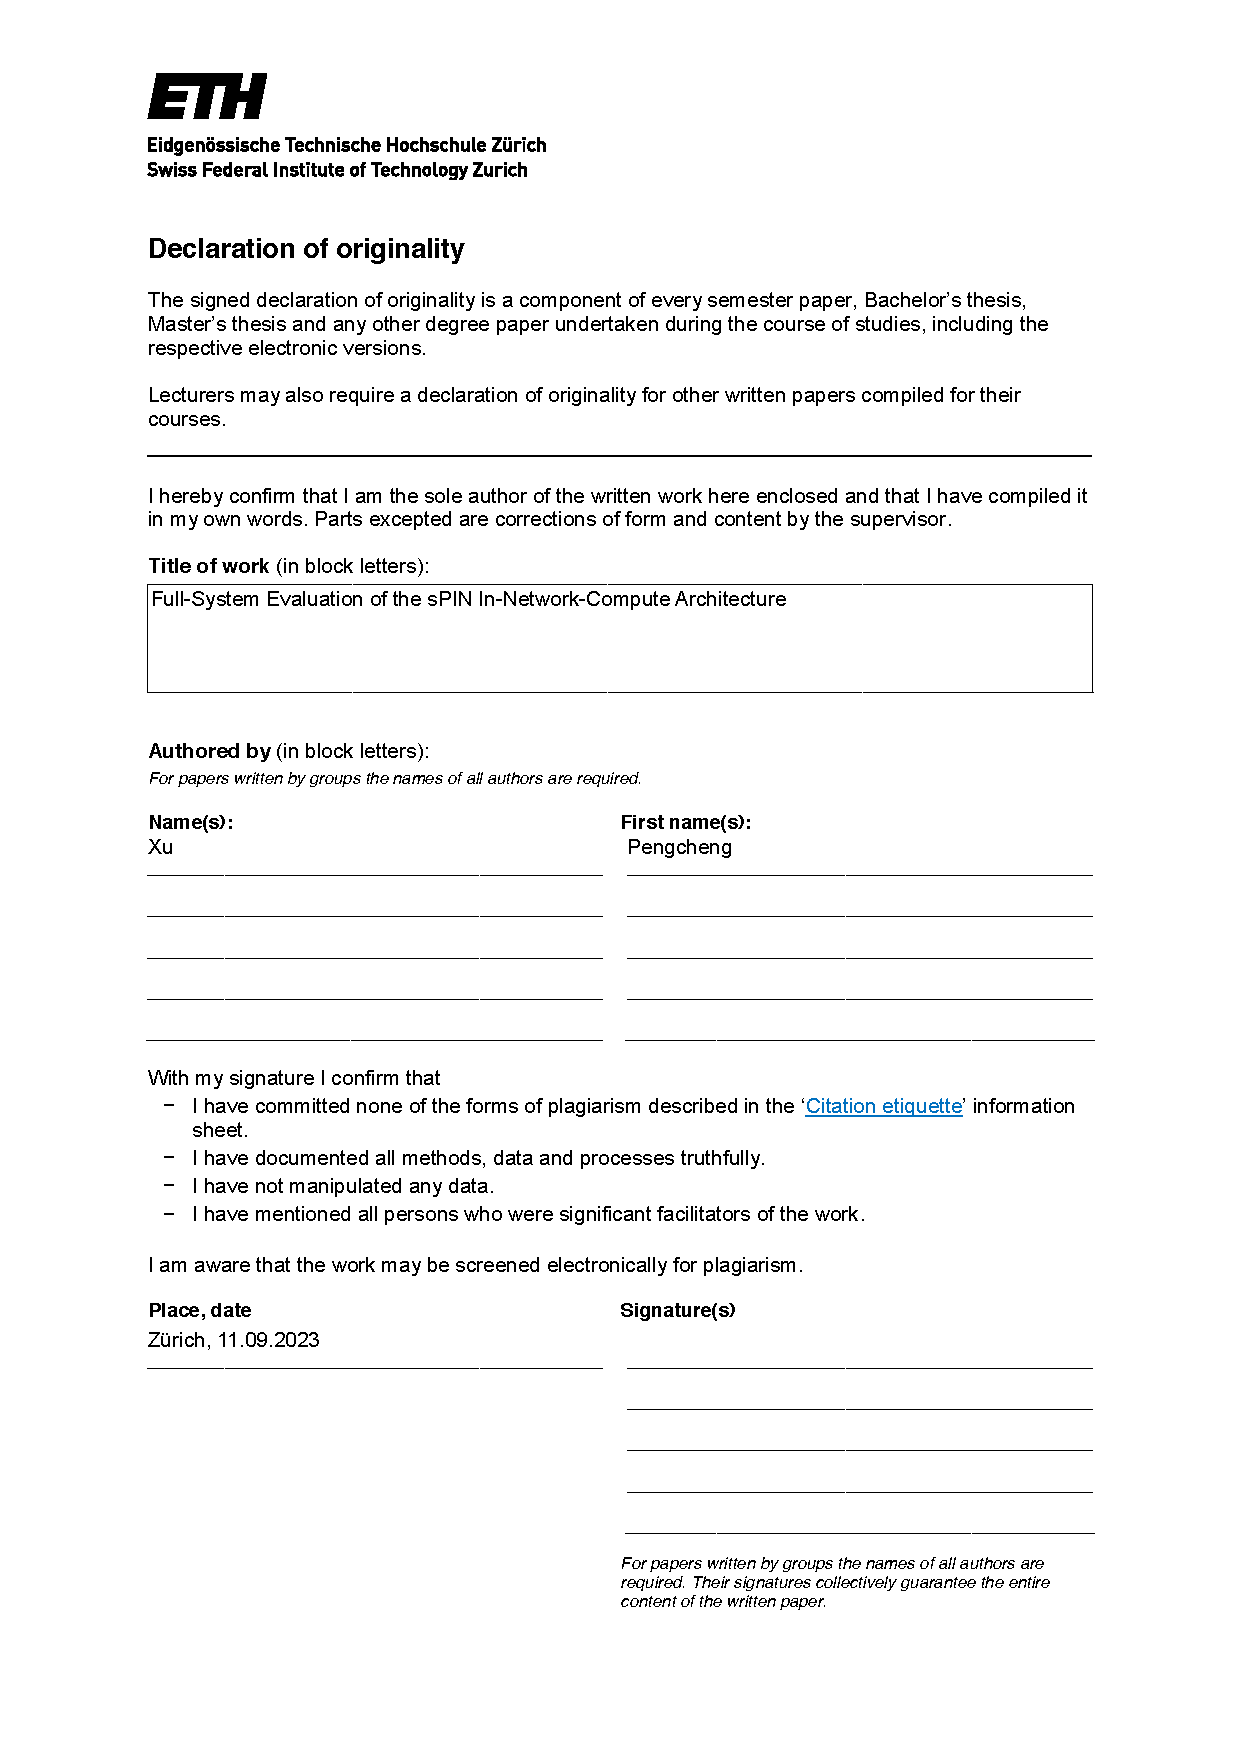
\includepdf[pages={-}]{declaration-originality.pdf}

\end{document}
